\chapter{Csatlakozó és bekötési rajzok}
A hétpólusú KF2510 csatlakozó számozása a nyomtatott áramköri lapon látható. A fénykép szerinti tájolást és az érintkezők számát használja, ne csak a vezetékszíneket. 1: K30/KL30, tápbemenet; 2: V2; 3: V1; 4: 1WRE, One-Wire; 5: KL, fenntartott K-Line; 6: +5 V kimenet, legfeljebb 30 mA; 7: GND, test.

A voltmérő kapcsolási rajza nevezi meg a fenntartott K-Line funkciót és az 5 V-os kimenet áramkorlátját. Az analóg bemenetek általános feszültséghatárai nincsenek megadva. A Check Engine alkalmazásnál szereplő 12 V nem jelenti azt, hogy más bemenetek is elviselik ezt. Mindig az adott érzékelő rajzát kövesse.

Az eredeti ábrák angol feliratai változatlanok; a kapcsolódó funkciókat ez az útmutató magyarul magyarázza el.

\begin{figure}[H]
\centering
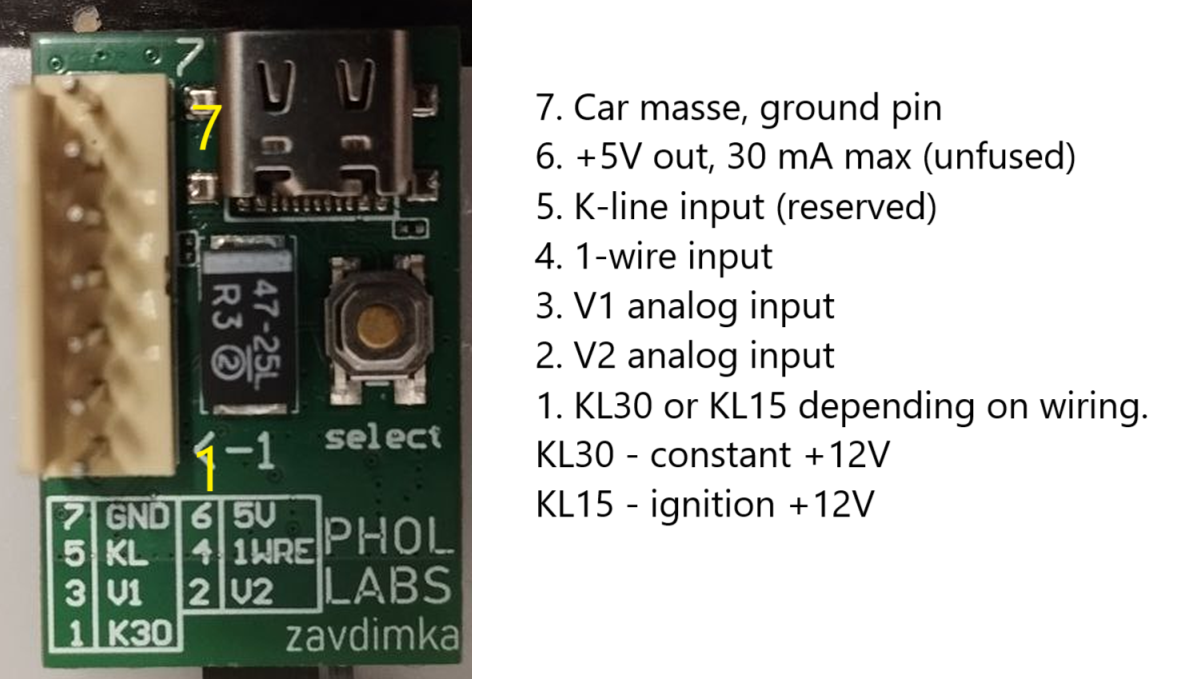
\includegraphics[width=.85\textwidth,height=.60\textheight,keepaspectratio]{figures/ivevo/image20.png}
\caption{Csatlakozó és bekötési rajzok}
\end{figure}
\clearpage
\section{Voltmérő}

\begin{figure}[H]
\centering
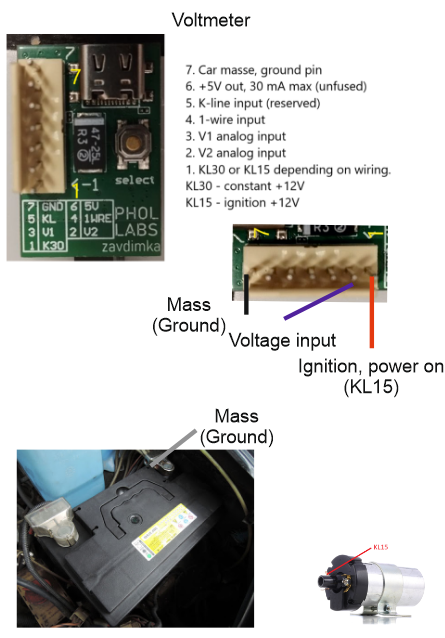
\includegraphics[width=.85\textwidth,height=.60\textheight,keepaspectratio]{figures/ivevo/image5.png}
\caption{Voltmérő}
\end{figure}
\clearpage
\section{Fokozatkijelző}

\begin{figure}[H]
\centering
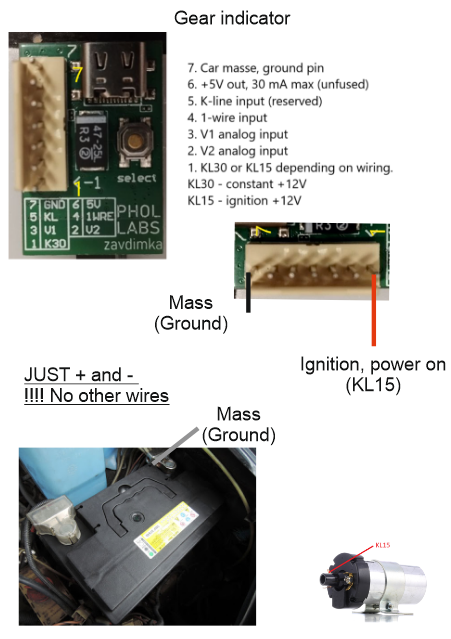
\includegraphics[width=.85\textwidth,height=.60\textheight,keepaspectratio]{figures/ivevo/image6.png}
\caption{Fokozatkijelző}
\end{figure}
\clearpage
\section{Olajnyomás}

\begin{figure}[H]
\centering
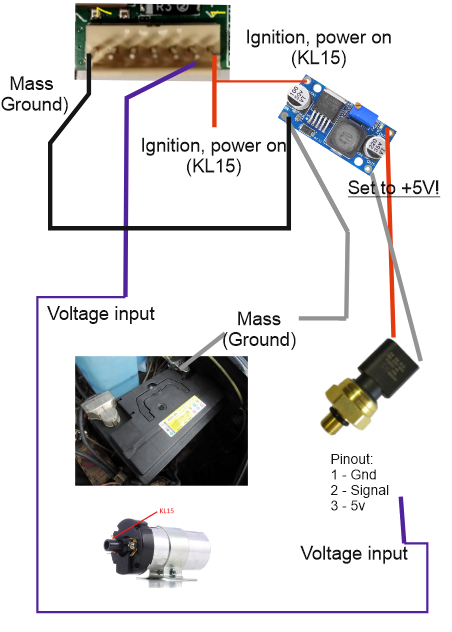
\includegraphics[width=.85\textwidth,height=.60\textheight,keepaspectratio]{figures/ivevo/image1.png}
\caption{Olajnyomás}
\end{figure}
\clearpage
\section{NTC-hőmérő}

\begin{figure}[H]
\centering
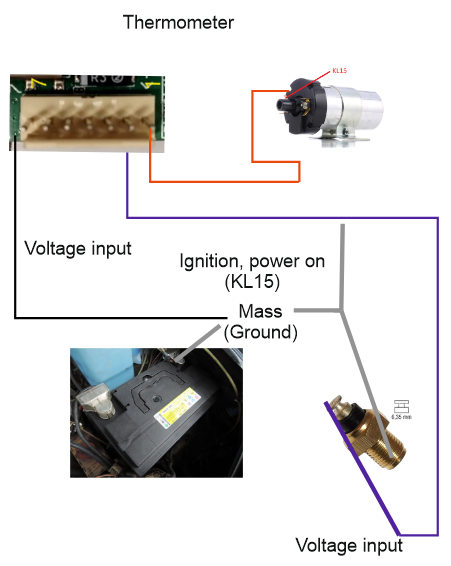
\includegraphics[width=.85\textwidth,height=.60\textheight,keepaspectratio]{figures/ivevo/image13.png}
\caption{NTC-hőmérő}
\end{figure}
\clearpage
\section{Digitális hőmérő}

\begin{figure}[H]
\centering
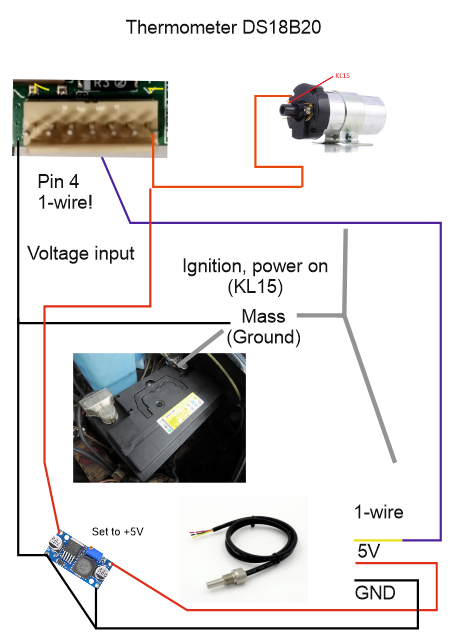
\includegraphics[width=.85\textwidth,height=.60\textheight,keepaspectratio]{figures/ivevo/image8.png}
\caption{Digitális hőmérő}
\end{figure}
\clearpage
\section{Szélessávú lambda}

\begin{figure}[H]
\centering
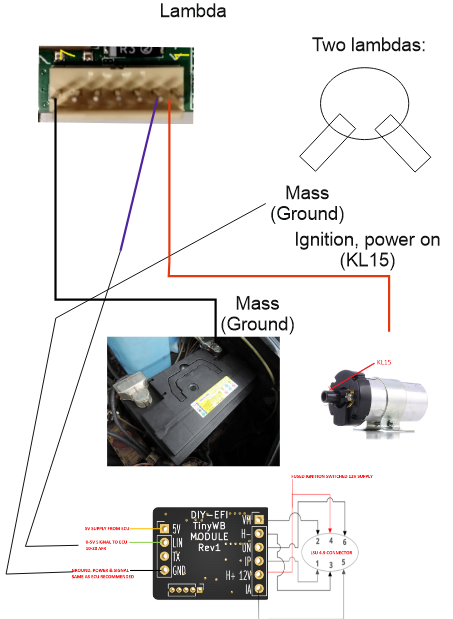
\includegraphics[width=.85\textwidth,height=.60\textheight,keepaspectratio]{figures/ivevo/image3.png}
\caption{Szélessávú lambda}
\end{figure}
\clearpage
\section{Töltőnyomás}

\begin{figure}[H]
\centering
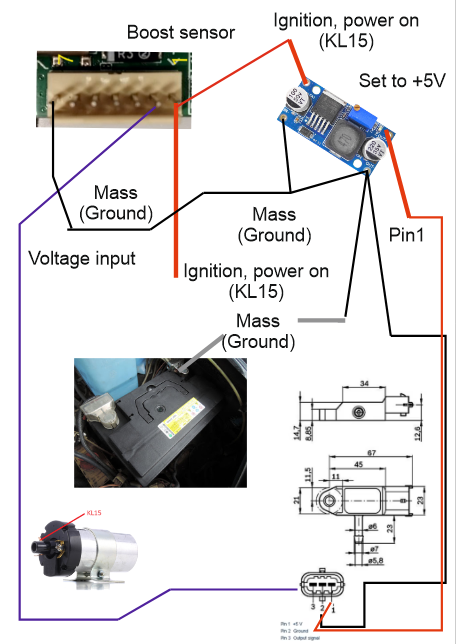
\includegraphics[width=.85\textwidth,height=.60\textheight,keepaspectratio]{figures/ivevo/image17.png}
\caption{Töltőnyomás}
\end{figure}
